\subsection{Explicacion del modelo}
    La implementación del MapReduce para resolver el problema esta basado en el
    siguiente esquema:\\
    \begin{figure}[ht]
        \begin{adjustbox}{addcode={
            \begin{minipage}{\width}}{
                \caption{Esquema de un map reduce}
            \end{minipage}},rotate=360,center}
            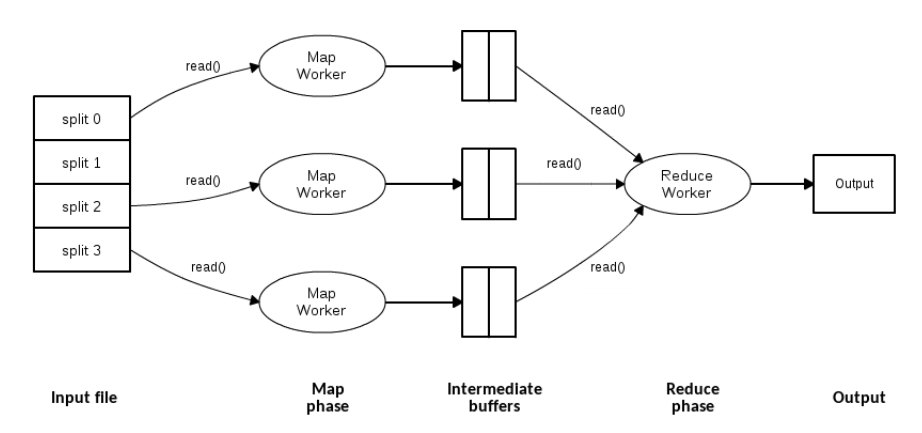
\includegraphics[scale=.6]{map_reduce_schema.png}
        \end{adjustbox}
    \end{figure}
    \FloatBarrier

    En nuestro caso creamos una clase llamada \code{MapReduce} la cual usa una
    libreria de \code{python} llamada \code{multiprocessing} en donde usamos el
    modulo \code{pool} el cual ofrece un medio conveniente para paralelizar la
    ejecución de una función a través de múltiples valores de entrada, distribuyendo
    los datos de entrada a través de procesos (paralelismo de datos).\\

    Entonces lo que hicimos fue instanciar dos \code{pool}, uno para hacer el map y
    el otro para el reduce de manera que el primero se le pasa como atributo la
    cantidad de worker en el cual se quiere paralelizar el problema y el segundo
    solo se usa uno de manera tal que la fase de reduce se la serie.

\subsection{Multiplicacion de matrices por bloques}

    \paragraph{Preprocesamiento}

        Generamos una lista de tuplas donde cada una tiene la posicion
        \code{r}, \code{c} de un bloque de la matriz A, tiene el bloque en
        custion \code{a\_block\_rc}, y la fila numero \code{c} de bloques de la
        matriz B, quedando con este formato: \\
        \code{(r, c, a\_block\_rc, b\_block\_c)}

    \paragraph{Mapeo}

        Recibimos la posicion \code{r}, \code{c} del bloque \code{a}, el bloque
        \code{a} y una lista de bloques \code{b} que es la fila \code{c} de
        bloques en la matriz B.\\
        Entonces multiplicamos el bloque \code{a} por cada bloque de la lista de
        bloques \code{b} y guardamos en un vector una tupla con una clave
        \code{r}, \code{c\_b} donde \code{c\_b} es el indice en la lista de
        bloques \code{b} y como valor guardamos la multiplicacion. Por cada
        multiplicacion, agregamos una de estas tuplas al vector de salida para
        luego devolver este.

    \paragraph{Reduccion}

        Recibimos la posicion de un bloque de salida y una lista de
        multiplicaciones parciales de bloques. Se suman estas multiplicaciones
        parciales y se devuelve un vector con los valores resultantes del la
        multiplicacion. Pero por cada valor se calcula la posicion de salida del
        mismo en la matriz resultante y nos deshacemos de la posicion de los
        bloques

\subsection{multiplicacion de matrices de elemento por fila}

    \paragraph{Preprocesamiento}

        Consiste en generar una lista de tuplas a partir de las dos matrices.
        Se itera por cada elemento (\code{a\_ij}) de la matriz A y se guarda
        en cada tupla el numero de fila del elemento \code{a\_ij}, el
        elemento \code{a\_ij} y la fila \code{j} de la matriz B.\\

    \paragraph{Mapeo}

        De esta manera, en la funcion map, obtenemos partes de esta lista de
        tuplas y devolvemos un par clave, valor donde la clave es la posicion
        de salida de la matriz resultante \code{(i, j)} y el valor es la
        multiplicacion del elemento \code{a\_ij} contra cada elemento de la
        fila \code{j} de la matriz B

    \paragraph{Reduccion}

        Obtenemos una posicion de salida y una lista de valores que resultaron
        de la multiplicacion que se hizo en el map. Entonces se suman las
        multiplicaciones parciales y se obtiene el valor en la posicion de salida
        de la matriz resultante

\subsection{Multiplicacion de matrices de columna por fila}

    \paragraph{Preprocesamiento}

        Consiste en generar una lista de tuplas a partir de las dos matrices.
        Se guarda en cada tupla la columna \code{i} de la matriz A y la fila
        \code{i} de la matriz B

    \paragraph{Mapeo}
        Recibimos una columna de la matriz A y una fila de la matriz B y por cada
        elemento de la columna \code{elem\_a} lo multiplicamos por cada elemento
        de la fila \code{elem\_b} obteniendo una matriz parcial de la
        multiplicacion. por cada multiplicacion guardamos en un vector una tupla
        con un par clave valor donde la clave es la posicion de salida de la matriz
        resultante y el valor es la multiplicacion anteriormente mencionada.
        Finalmente se devuelve el vector de tuplas.

    \paragraph{Reduccion}

        Se recibe la posicion de salida de la matriz resultante y una lista de
        multiplicaciones parciales. Entonces se suman estas y se devuelve la
        posicion de salida y la suma.



\subsection{Forma de ejecucion}
    Para el caso de Amdahl multiplicamos dos matrices de 10x10
    con 1, 2, 4, 8, 16 y 32 threads.\\

    Para el caso de gustafson se usan siempre 4 threads multiplicando dos matrices
    de 2x2, 4x4, 8x8, 16x16, 32x32 y 64x64\\

    Para realizar el calculo se debe ejecutar: \\
    \lstinline[columns=fixed]{$ sh scripts/run.sh}.\\

    Luego para generar los graficos que vemos en el informe se debe
    ejecutar: \\
    \lstinline[columns=fixed]{$ sh scripts/generate_output_data.sh}

\subsection{Datos sobre la computadora que se utilizó}
    El equipo sobre el que se realizarán las mediciones es una laptop con un
    procesador Intel core I7 que posee 4 nucleos a 2.7 Ghz, es decir, soporta
    hasta 4 threads en paralelo, con 16 Gb de memoria y corriendo sobre un
    sistema Linux.\\
    Para averiguar estos datos en linux se ejecutaron los siguientes comandos:\\
    \begin{itemize}
        \item Cantidad de cores: \lstinline[columns=fixed]{$ grep -c processor /proc/cpuinfo}
        \item Velocidad de reloj: \lstinline[columns=fixed]{$ lscpu | grep GHz}
        \item Memoria RAM: \lstinline[columns=fixed]{$ free -g}
    \end{itemize}